\documentclass[../main.tex]{subfiles}

\begin{document}

\chapter{Transcriptomic analysis of plasmodesmatal response to fungal chitin}
\label{cha:transcripts}

\section{Introduction}
It is well established that plasmodesmata react and respond to microbe presence
through the recognition of highly-conserved microbe associated molecular
patterns (MAMPs) by pattern recognition receptors (PRRs)
\cite{zipfelPlantPatternrecognitionReceptors2014a,
  chevalPlasmodesmalRegulationPlant2018}. One specific interaction of a protein
and a ligand which has been identified is between fungal chitin and CHITIN
ELCITOR RECEPTOR KINASE 1 (CERK1) \cite{miyaCERK1LysMReceptor2007}, where it has
been reported that CERK1 acts a receptor specific to chitin signalling (figure
\ref{fig:receptors}). Interestingly, it has been show that CERK1 is not a
requirement for plasmodesmatal closure in response to chitin and that another
protein, LYSIN MOTIF DOMAIN-CONTAINING GLYCOSYLPHOSPHATIDYLINOSITOL-ANCHORED
PROTEIN 2 (LYM2), is essential for a plasmodesmata; defence response to chitin
\cite{Faulkner2013} (figure: \ref{fig:receptors}).

As eluded to by \citet{Faulkner2013} the there
exists at least two (seemingly) independent signalling pathways involved in
chitin-triggered defence response in plants. Here, we present the outcome and
analysis of data created in collaboration with the Faulkner group which has
provided new insight into the behaviour of the LYM2 and CERK1 pathways in
Arabidopsis.


\begin{figure}[ht]
  \centering
  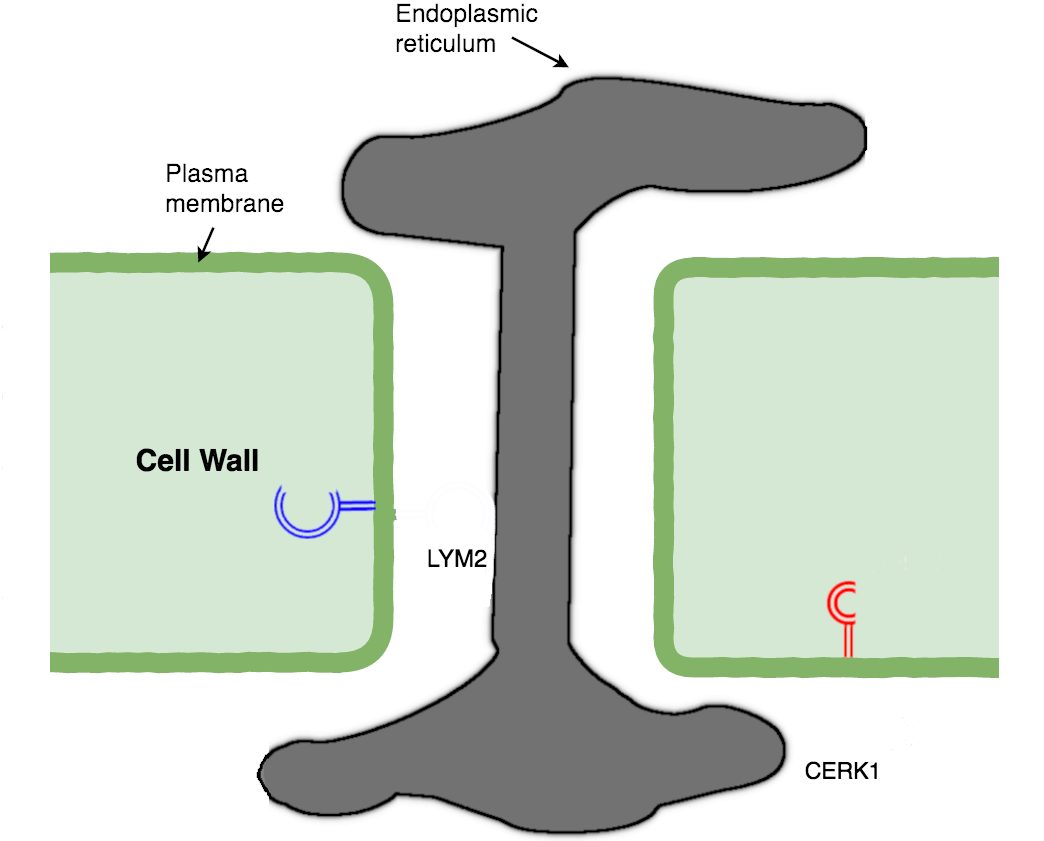
\includegraphics[width=0.5\columnwidth]{figures/original desmotubule.png}
  \caption[Plasmodesmata, \textit{lym2-1} and\textit{cerk2-1}diagram]{\label{fig:receptors}
    An illustrated plasmodesmata channel, with two
    known proteins involved in chitin signalling and plasmodesmata response. Red
    showing the canonical chitin detector CERK1, and in blue LYM2 a
    plasmodesmata localised protein}
\end{figure}

\section{Materials and methods}

\subsection{Plant materials}
An RNA-seq assay was performed on three genotypes of Arabidopsis Thaliana to
test for transcripts unique to chitin perception. Col-0 used as a control,
as well as \textit{lym2-1} and \textit{cerk2-1} which are knock-out mutants of
their respective chitin perception proteins. 

All three of these genotypes were grown \textit{in vitro}, as seedlings they
were introduced to one of two treatments. Either chitin or water solutions were
added and mixed into their suspension. Samples were taken at 30 minutes post
treatment and at 6 hours. Whole seedlings were taken and pooled and sequenced
together for robustness. Three replicates of each genotype, treatment and time
point were produced.


\subsection{Computational methods}

Data were pre-processed firstly through removing adaptor sequences, with
\textit{trimmomatic} \cite{bolgerTrimmomaticFlexibleTrimmer2014}. Sanity checks
were performed using \textit{fastqc} \cite{andrewsBabrahamBioinformaticsFastQC}.
Alignment was carried out using a combination of \textit{samtools} and
\textit{hisat2} \cite{liSequenceAlignmentMap2009}. Finally, \textit{htseq-count}
was used to prepare sequence counts from trimmed and aligned RNA-seq data
\cite{kimHISATFastSpliced2015}. Preparation of count data used the method
described by \citet{loveModeratedEstimationFold2014a} and normalised transcript
counts were created using \textit{DESEQ2}
\cite{piperCountNormalizationDESeq22017}.

With these normalised data, we calculated the false discovery rate (FDR) value
for chitin compared to water treatments of each genotype at each time point. We
specified that all genes with an FDR$< 0.05$ would be considered significant.
For further down-stream gene-ontology (GO) analysis we used
\cite{klopfensteinGOATOOLSPythonLibrary2018}, and further limited genes of
interest to having a Log2 Fold Change (LFC) of $>2$ to select only genes with a
high degree of difference from their water treatment.

\section{Analysis of chitin response after 30 minutes}
\label{sec:seqresults}

\subsection{Col-0 and \textit{lym2-1} respond strongly to chitin}

Initial analysis indicates that at our earliest time point, 30 minutes post
treatment, a significant response to chitin is seen in both Col-0 and
\textit{lym2-1}. Unsurprisingly, \textit{cerk2-1} produced only 3 differentially
expressed genes (DEGs) whereas Col-0 and \textit{lym2-1} show to have 3664 and
5196 respectively (figure: \ref{fig:05hrDEGs}). A surprising result is seen in that the
\textit{lym2-1} mutant had a much higher level of mis-regulation following
chitin treatment of $\approx70\%$ more genes classified as significantly different
than the control.

\begin{figure}[ht]
  \centering
  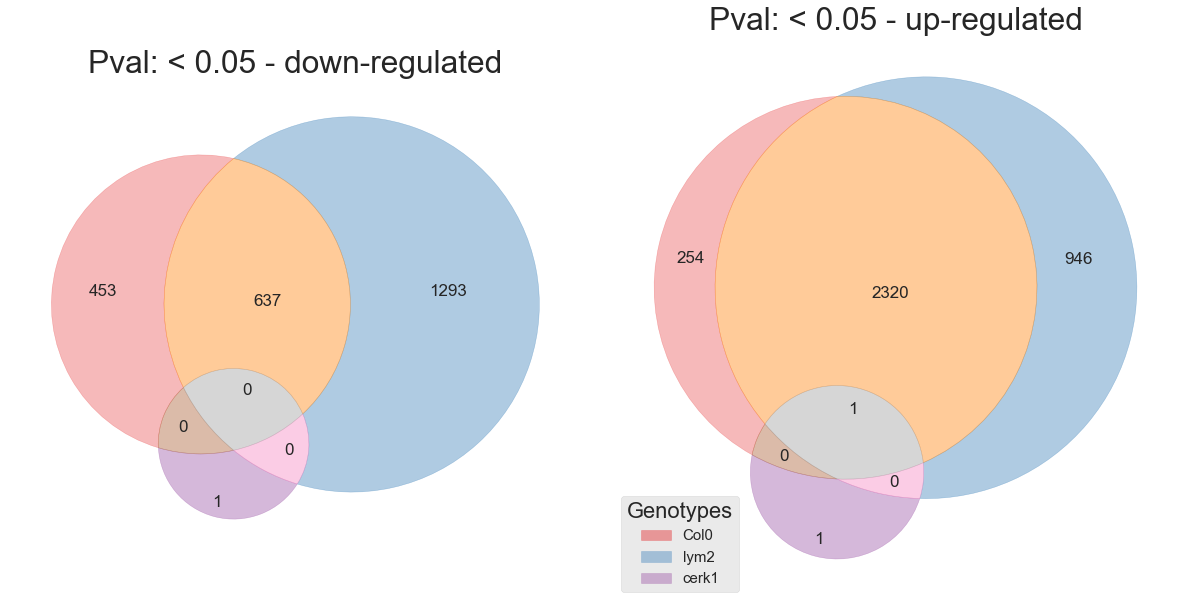
\includegraphics[width=0.8\columnwidth]{figures/vennTreatmentschitin.png}
  \caption[Venn diagram of differential genes 30 minutes post-chitin treatment]{\label{fig:05hrDEGs} Venn diagram of differential genes for Col-0,
    \textit{cerk2-1} and \textit{lym2-1} 30 minutes after exposed to chitin}
\end{figure}

\subsection{\textit{cerk2-1} is required for a substantial transcriptional response to chitin}

Comparing the most DEGs for each genotype reveals that a similar expression
profile is seen in up-regulated genes for both Col-0 and \textit{lym2-1} , while
\textit{cerk2-1} doesn't show any genes that would be classified as having a
substantially different expression compared with the water control (DEGs with
greater than 2 LFC, three genes found in \textit{cerk2-1} have a small degree of
regulation) (figure: \ref{fig:DEG5}). In genes down-regulated at 30
minutes post-treatment, \textit{lym2-1} and Col-0 have a slight difference.
Overall at this time point \textit{lym2-1} shows a much higher degree of
mis-regulation (figure: \ref{fig:05hrDEGs}). This behaviour may suggest that
missing a key piece of plasmodesmata signalling leads to the inability to
correctly contain and regulate gene expression.

\begin{figure}[!ht]
  \centering
  \subfloat[Most up-regulated genes at 30 minutes post-treatment of chitin.
  \label{subfig-2:deg5}]{%
    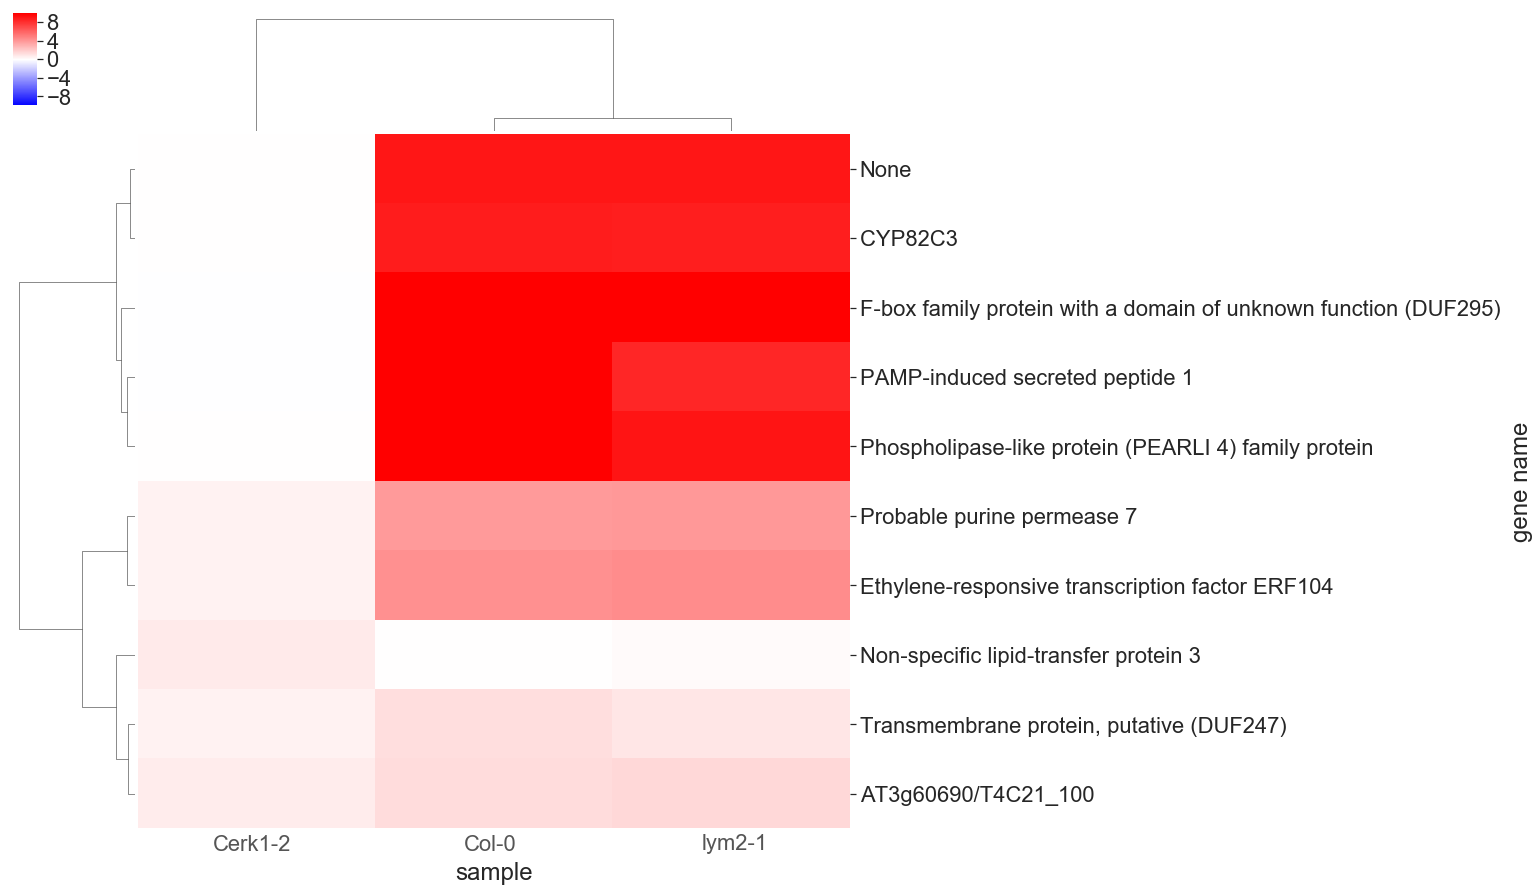
\includegraphics[width=1\columnwidth]{./figures/chitin_water_05hr_up.png}
  }
  \\
  \subfloat[Most down-regulated genes at 30 minutes post-treatment of chitin\label{subfig-1:deg5}]{%
    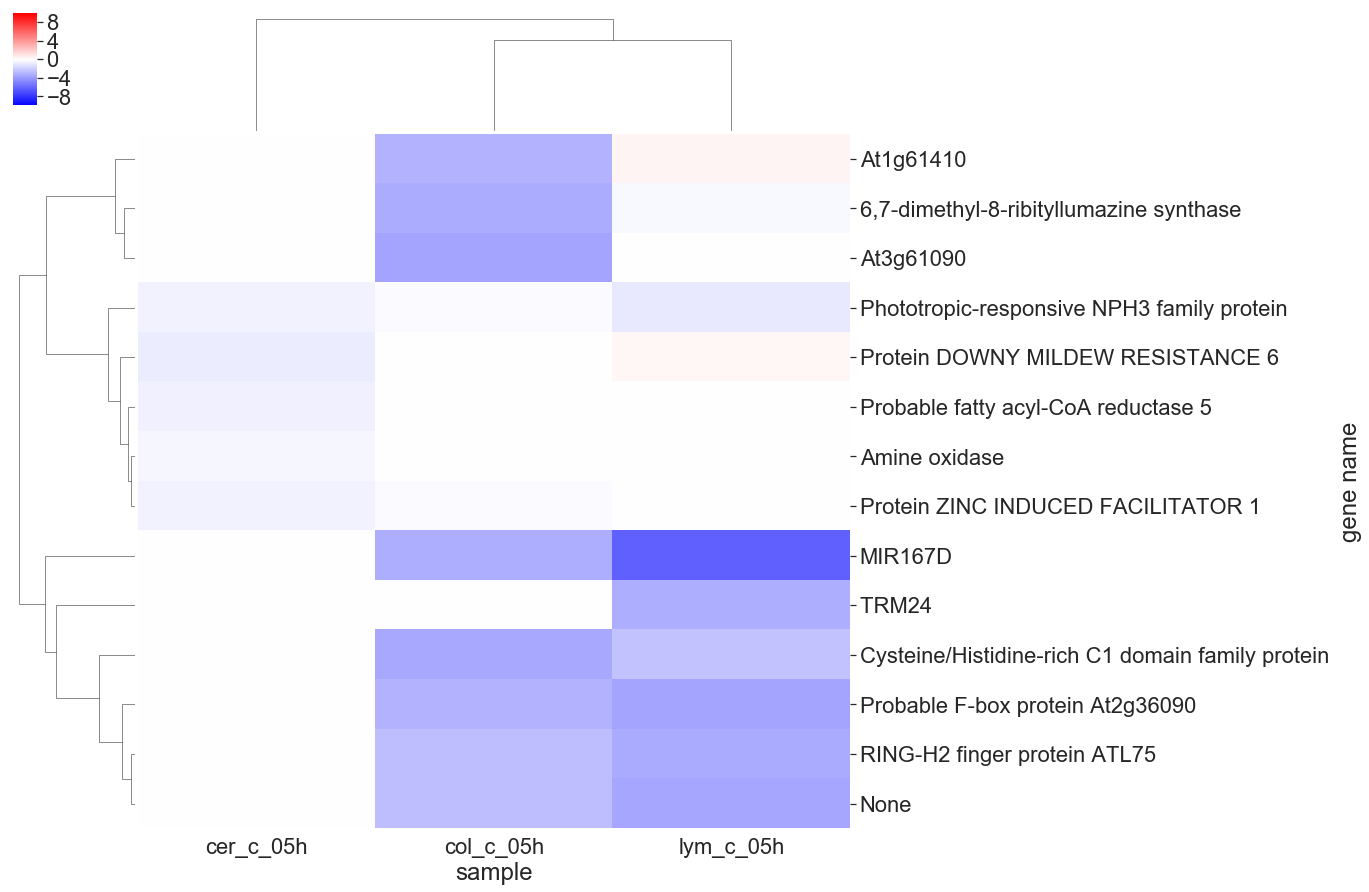
\includegraphics[width=1\columnwidth]{./figures/chitin_water_05hr_down.png}
  }
  \caption[Most differential genes at 30 minutes post-chitin treatment]{5 most up and down regulated genes at 30 minutes post chitin
    treatment for each genotype. Columns show each genotype tested, colour intensity represents LFC}
  \label{fig:DEG5}
\end{figure}


\subsection{\textit{cerk1-2} produces a minor response to chitin}

Of the several thousand DEGs found in this study only three have been shown to
affect \textit{cerk2-1}. AT5G24530 (DMR6) is shown to be uniquely down-regulated when
presented with chitin. Curiously, this gene has previously been described as
enhancing susceptibility to downy mildew \cite{DOWNYMILDEWRESISTANT}, these data
could suggest that a secondary fallback mechanism is activated only when CERK1 is
not present (figure: \ref{subfig-1:cerk}).

Two other genes that appear to be differentially regulated in \textit{cerk2-1}
AT5G59320 (LTP3) and AT3G60690 (SAUR59) may be worth further consideration. LTP3
has been shown to be involved with abscisic acid, an important signalling
molecule in abiotic stress \cite{vishwakarmaAbscisicAcidSignaling2017} and
SAUR59 is indicated to be a highly mobile transcript
\cite{thiemeEndogenousArabidopsisMessenger2015} and thus potentially involved in
cell-cell communication of stress (Figures \ref{subfig-2:cerk} and
\ref{subfig-3:cerk}).

%  This indicates that chitin perception is not wholly dependant
% on CERK1, as previously thought.  


\begin{figure}[!ht]
  \subfloat[AT5G24530 (DMR6), the single gene found in \textit{cerk1-2} mutants
  which shows a down-regulation in response to chitin \label{subfig-1:cerk}]{%
    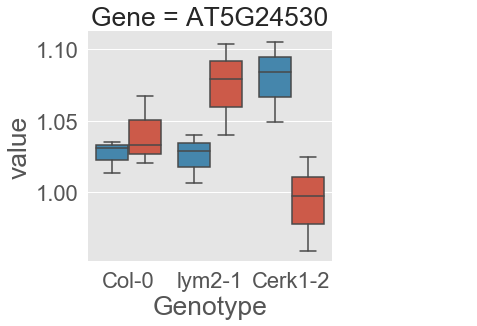
\includegraphics[width=0.45\columnwidth]{./figures/cerk_genes_AT5G24530.png}
  }
  \qquad 
  \subfloat[AT5G59320 (LTP3), Significantly up-regulated in \textit{cerk1-2}
  but not in Col-0 or \textit{lym2-1} \label{subfig-2:cerk}]{%
    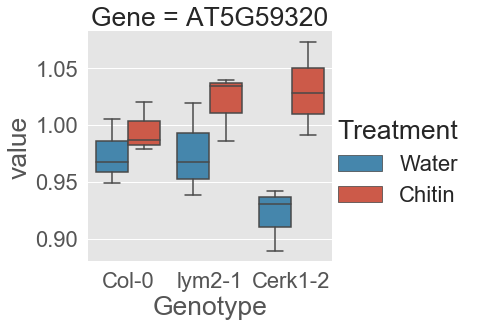
\includegraphics[width=0.45\columnwidth]{./figures/cerk_genes_AT5G59320.png}
  }\\
  \subfloat[AT3G60690 (SAUR59), Significantly up-regulated in response to
  chitin for all genotypes in study \label{subfig-3:cerk}]{%
    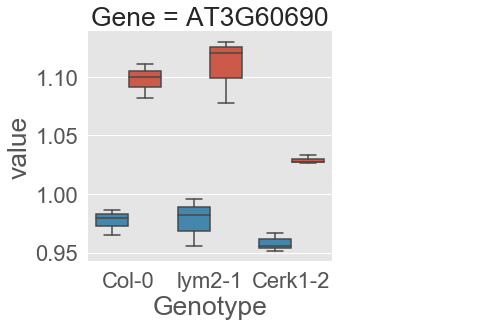
\includegraphics[width=0.45\columnwidth]{./figures/cerk_genes_AT3G60690.png}
  }
  
  \caption[Differential \textit{cerk1-2} genes at 30 minutes post-chitin treatment]{Genes which were found to have a differential regulation in the
    \textit{cerk1-2} genotype. Presented for comparison are the values in both
    Col-0 and \textit{lym2-1}, Y values are given as normalised transcript counts
    for each transcript across different treatments (Normalisation was performed
    gene-wise, values are comparative across treatments but not between genes).
    Blue colour in boxplots represents water treatments, red as chitin }
  \label{fig:cerk}
\end{figure}

As these data indicate that the effect of knocking-out CERK1 is highly specific,
we hypothesise that CERK1 acts at a high-level and that its absence
inhibits many downstream processes, such as those we see in Col-0 and \textit{lym2-1}.
Our data also maintain and strengthen the established theory that CERK1 and LYM2 are
independent signalling pathways \cite{Faulkner2013, miyaCERK1LysMReceptor2007,
  narusakaPresenceLYM2Dependent2013}.



\subsection{Gene ontology analysis shows Col-0 and \textit{lym2-1} have similar
  disruption patterns}

To better ascertain the transcriptional changes observed in \textit{lym2-1} we
performed Gene ontology (GO) term analysis on the DEGs found. Whilst having
hundreds of differential genes both Col-0 and \textit{lym2-1} have some curious
similarities. Firstly, they show very few GO-terms being enriched/purified.
Secondly they show a great deal of overlap.

This analysis indicates that a large part of the transcriptomic disruption
caused by chitin results in seemingly disconnected processes (thus the low
number of significant GO terms). The terms which do create interest are
``response to chitin'' which indicates that Col-0 has a sub-set of DEGs that are
down-regulated exclusively (figure \ref{fig:05hrGO}), and ``defense response to bacterium''
which conversely shows an exclusive set of \textit{lym2-1} genes that are
down-regulated (supplemental
tables \ref{cha:suppltbl}).

However, closer investigations reveals that expression profiles of these groups
are similar and that repeated experiments could give contradictory results
(supplemental figures \ref{fig:respchitin} and \ref{fig:defbacterium}).


\begin{figure}[ht]
  \centering
  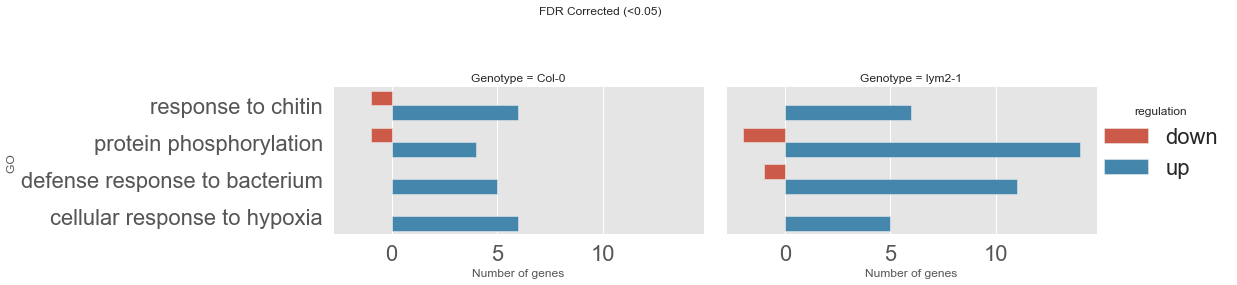
\includegraphics[width=\columnwidth]{figures/05hrGO.png}
  \caption[GO terms found in Col-0 and \textit{lym2-1} at 30
    minutes post chitin treatment]{\label{fig:05hrGO} GO terms found in Col-0 and \textit{lym2-1} at 30
    minutes post chitin treatment. Up-regulated terms are given as blue and down
  in red. Down-regulated terms are shown as negative values to indicate that the
  respective term has genes which are down-regulated}
\end{figure}


\clearpage

\section{Analysis of chitin response after 6 hours}

\subsection{Col-0 sustains high number of DEGs 6 hours post chitin application}
\label{sec:col-0-sustains}

As previously shown the number of DEGs found at 30 minutes post chitin treatment
was high for both Col-0 and \textit{lym2-1}, with the latter showing higher
numbers of differential genes. After 6 hours we see that this reverses (figure
\ref{fig:6hrDEGs}). Our results show that whilst diminished, Col-0 has a large
number of genes (over 1500) differentially regulated at this time-point. Whereas
\textit{lym2-1} has shown its response drastically drops off compared with its
previous, 30 minute time-point and here gives just 366 DEGs. 


\begin{figure}[ht]
  \centering
  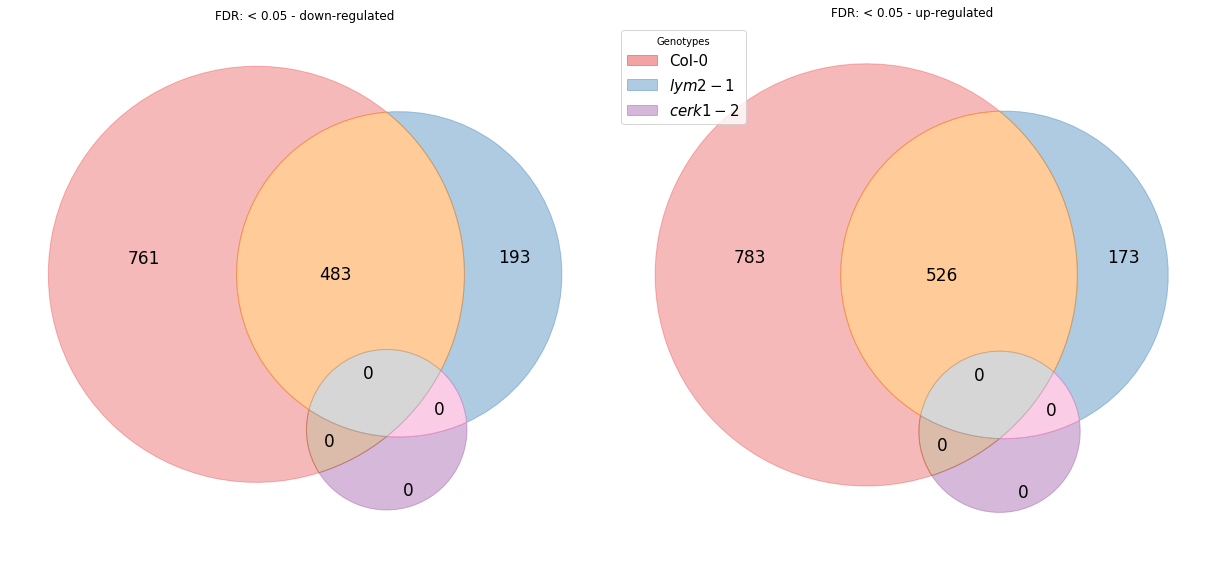
\includegraphics[width=0.8\columnwidth]{figures/vennTreatmentschitin6.png}
  \caption{\label{fig:6hrDEGs} Differentially expressed genes Venn diagram at 30
  minutes post-chitin treatment}
\end{figure}

Unsurprisingly, \textit{cerk1-2} displays an almost complete disregard for
chitin treatments 6 hours after exposure (figure: \ref{fig:DEG6}). Though this
gives further evidence that CERK1 allows for organisation of downstream
processes. 


\begin{figure}[!ht]
  \centering
  \subfloat[5 most up-regulated genes for each genotype \label{subfig-1:deg6}]{%
    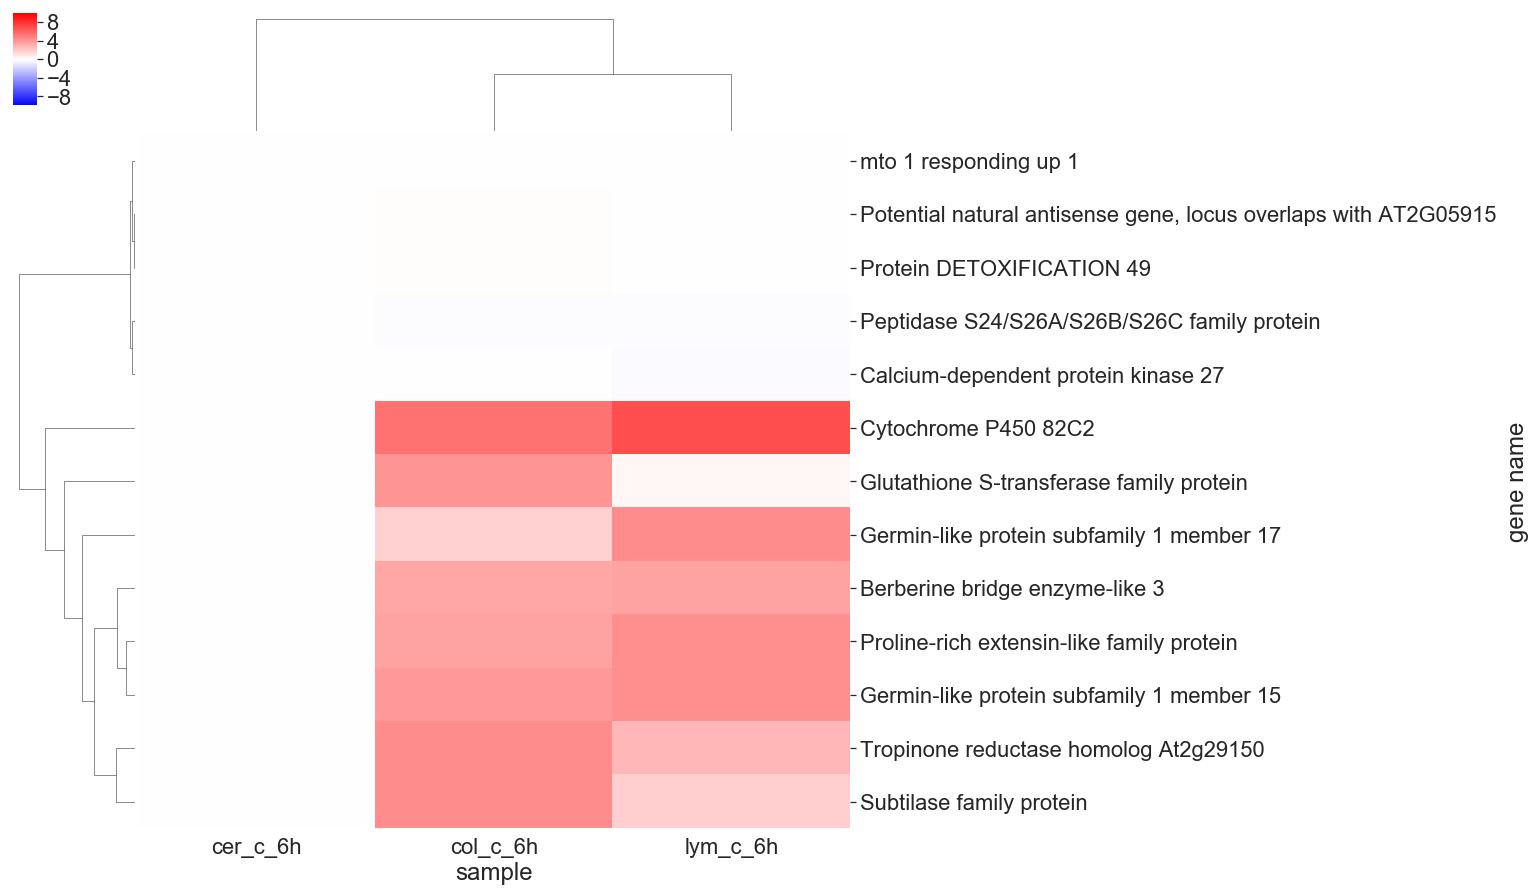
\includegraphics[width=1\columnwidth]{./figures/chitin_water_6hr_up.png}
  }
  \\
  \subfloat[5 most down-regulated genes for each genotype\label{subfig-2:deg6}]{%
    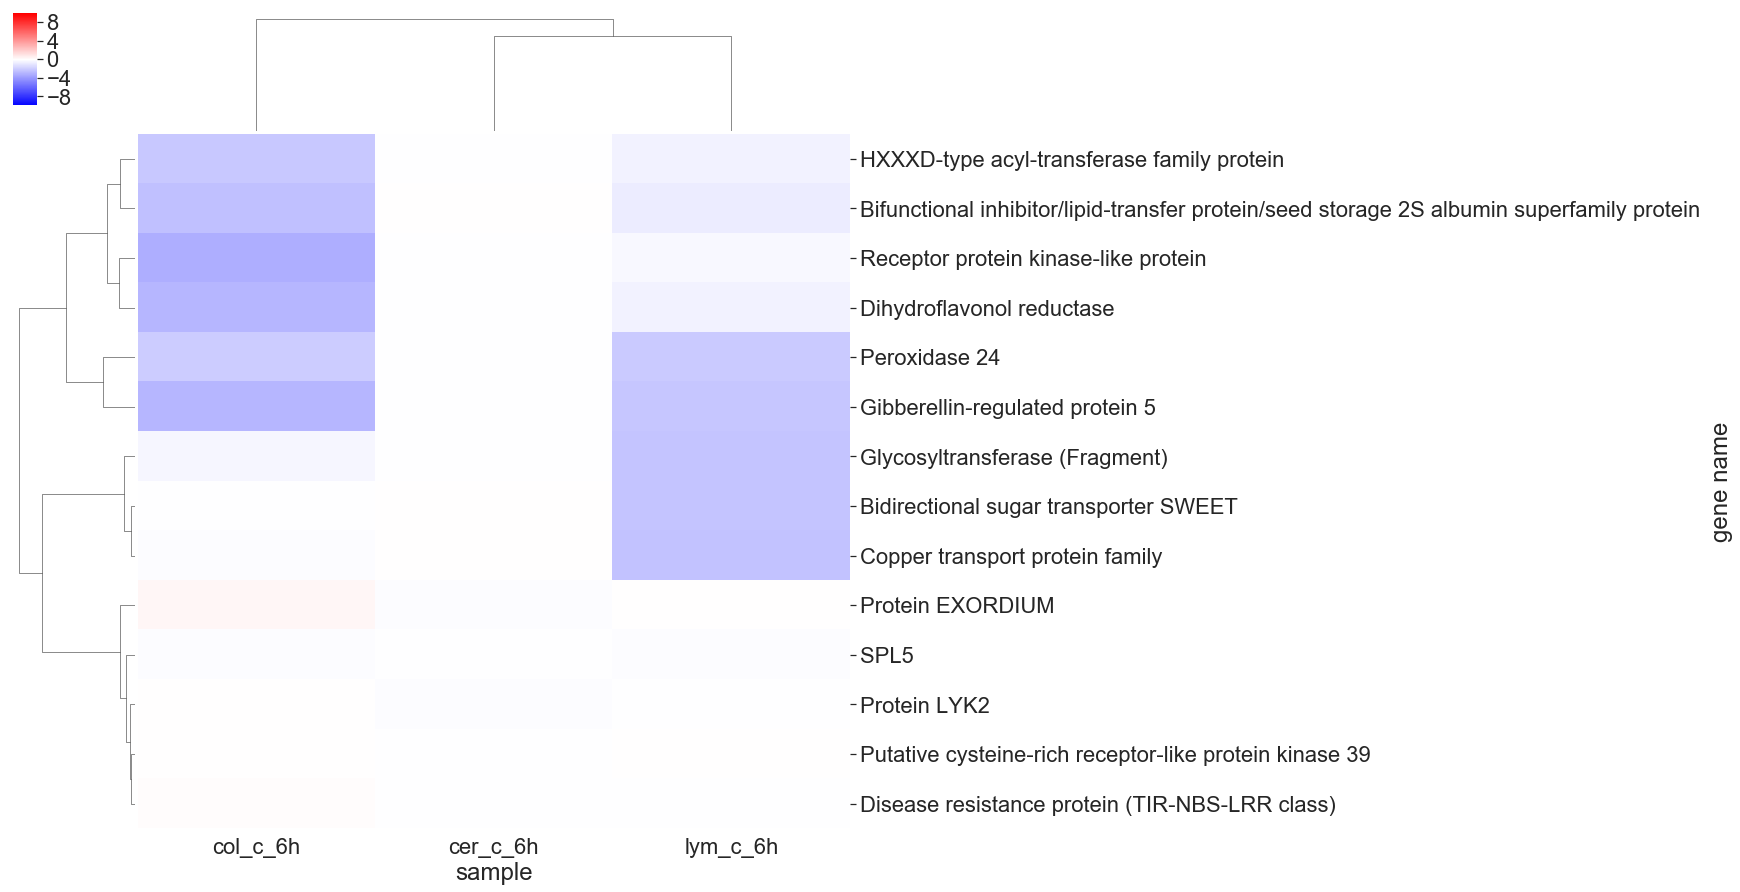
\includegraphics[width=1\columnwidth]{./figures/chitin_water_6hr_down.png}
  }
  \caption{Most up/down regulated genes for each genotype 6 hours post chitin application}
  \label{fig:DEG6}
\end{figure}



\subsection{Response to chitin by CERK1 and LYM2 occurs early in the defence
  process}
\label{sec:resp-chit-cerk1}

Given that plasmodesmata response to chitin can occur from 30 minutes
post-application \cite{chevalChitinPerceptionPlasmodesmata2019} and that
systemic response to fungal pathogens occurs 48-72 hours after initial
infections \cite{gaoSignalRegulatorsSystemic2015}, we suggest that CERK1 and
LYM2 may manage and enable early processes that go on to produce larger scale
defence responses and thus are critical to enabling systemic acquired
resistance. Our data supports this suggestion, as we see a strong drop-off of
DEGs for \textit{cerk1-2} and \textit{lym2-1} between 30 minutes and 6 hours
after chitin application (figure: \ref{fig:tmpHist})


\begin{figure}[!ht]
  \centering
  \subfloat[30 minutes post chitin application\label{subfig-1:tmpHist}]{%
    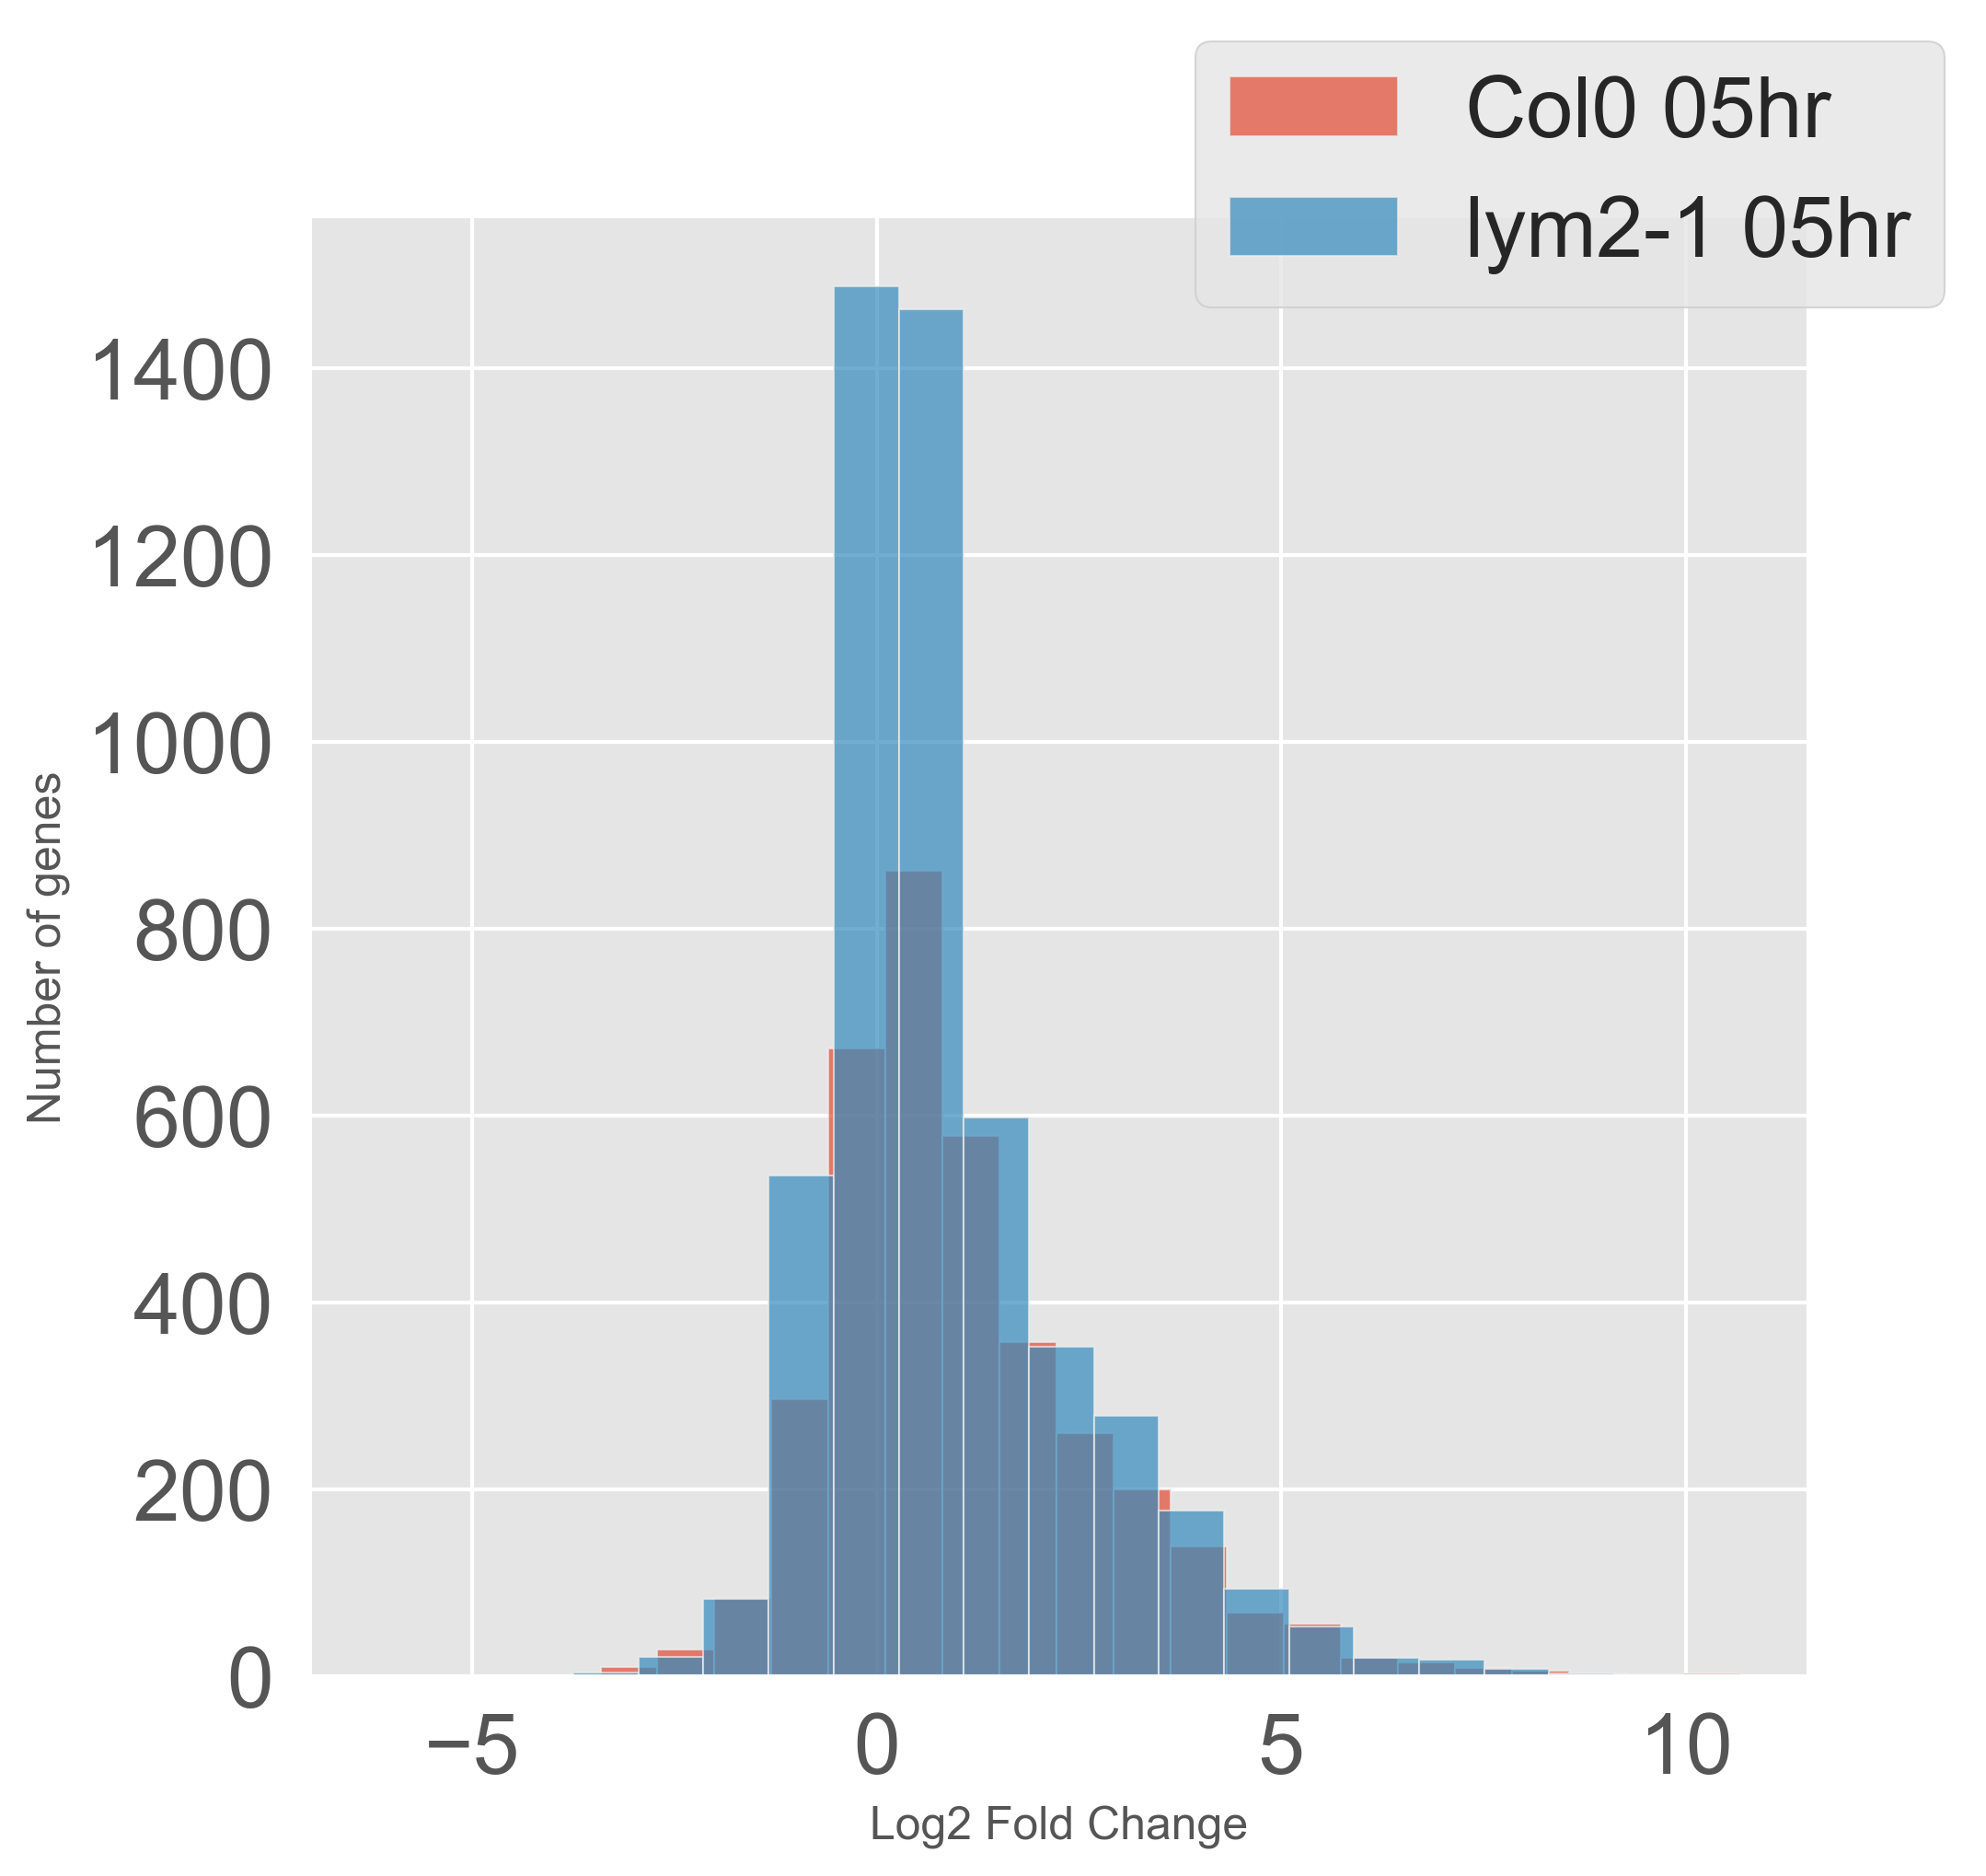
\includegraphics[width=0.6\columnwidth]{./figures/hist05hr.png}
  }
  \\
  \subfloat[6 hours post chitin application\label{subfig-2:tmpHist}]{%
    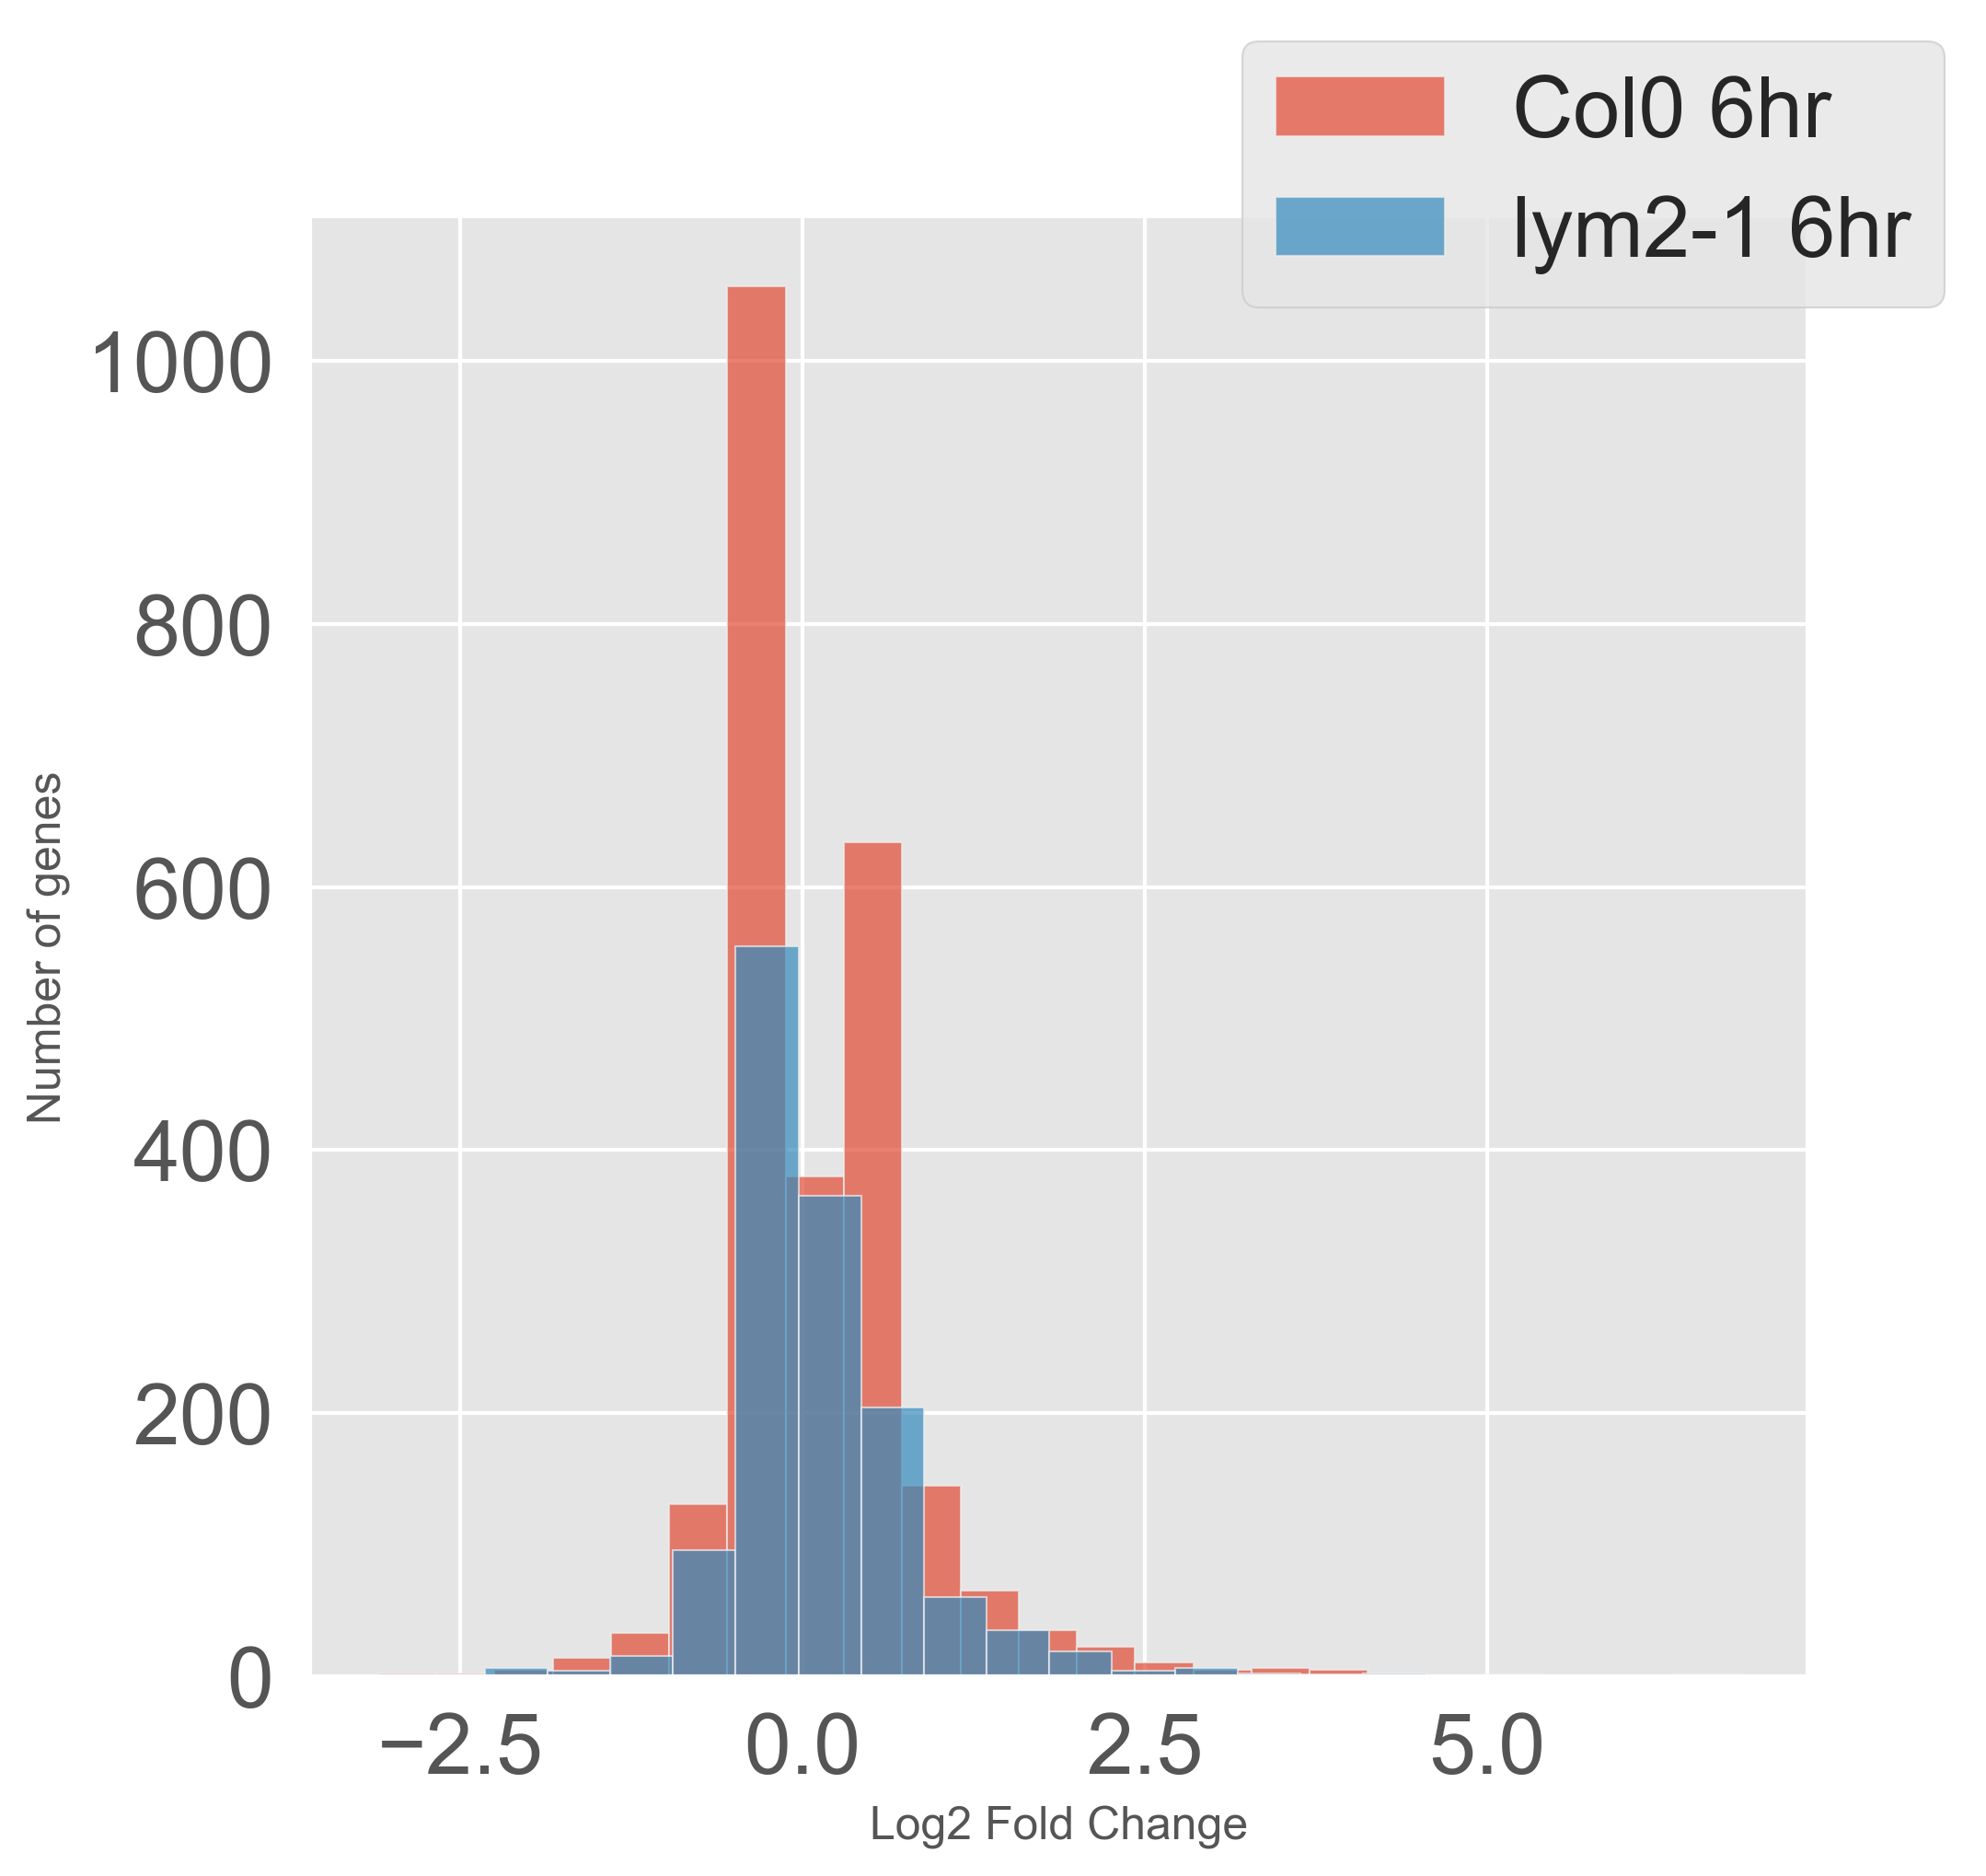
\includegraphics[width=0.6\columnwidth]{./figures/hist_6hr.png}
  }
  \caption[Temporal histograms of RNAseq data]{Temporal histograms. In red Col-0 DEGs are shown, \textit{lym2-1} in
    blue. Positive values show up-regulation and negative down in response to
    chitin treatments}
  \label{fig:tmpHist}
\end{figure}

\subsection{Plasmodesmatal closure depends on LYM2}
\label{sec:plasm-clos-depends}

As previously shown by \citet{Faulkner2013}, LYM2 is required for a
plasmodesmatal response to chitin and that CERK1 is not entirely necessary. The
results presented by these transcriptional data would initially cause confusion
on the \textit{lym2-1} response compared to \textit{cerk1-2}. However, as we
show that \textit{lym2-1}'s response quickly fades (figure: \ref{fig:tmpHist}),
we could conclude that LYM2 is not required for chitin perception, but it is
explicitly required for a plasmodesmatal defence response.

\clearpage

\section{Analysis of temporally different genes}
\label{sec:tempexpress}

\subsection{Searching for genes with unique temporal regulation}
\label{sec:col-0-textitlym2}

With many hundreds of genes differentially expressed in both \textit{lym2-1}
and Col-0 we wanted a method that could extract and find genes which may be of
special interest. To that end we developed a method for finding genes which had
opposing behaviours across both of the time-points we sequenced. For example we
would consider a gene interesting if it was down-regulated at 30 minutes after
chitin treatment and up-regulated at 6 hours after. To further reduce the number
of genes that we specified those which had also been differentially regulated
with a value of 2 or greater log fold change (LFC).

Without applying this method, we found too many individual genes to study
(figure: \ref{subfig-1:diverg}), though after we found a more manageable amount
(figure: \ref{subfig-2:diverg}). Here we present two genes of interest, one
selected using this method from Col-0 and another from \textit{lym2-1}.

\begin{figure}[!ht]
  \centering
  \subfloat[Genes found when selecting for FDR < 0.05 \label{subfig-1:diverg}]{%
    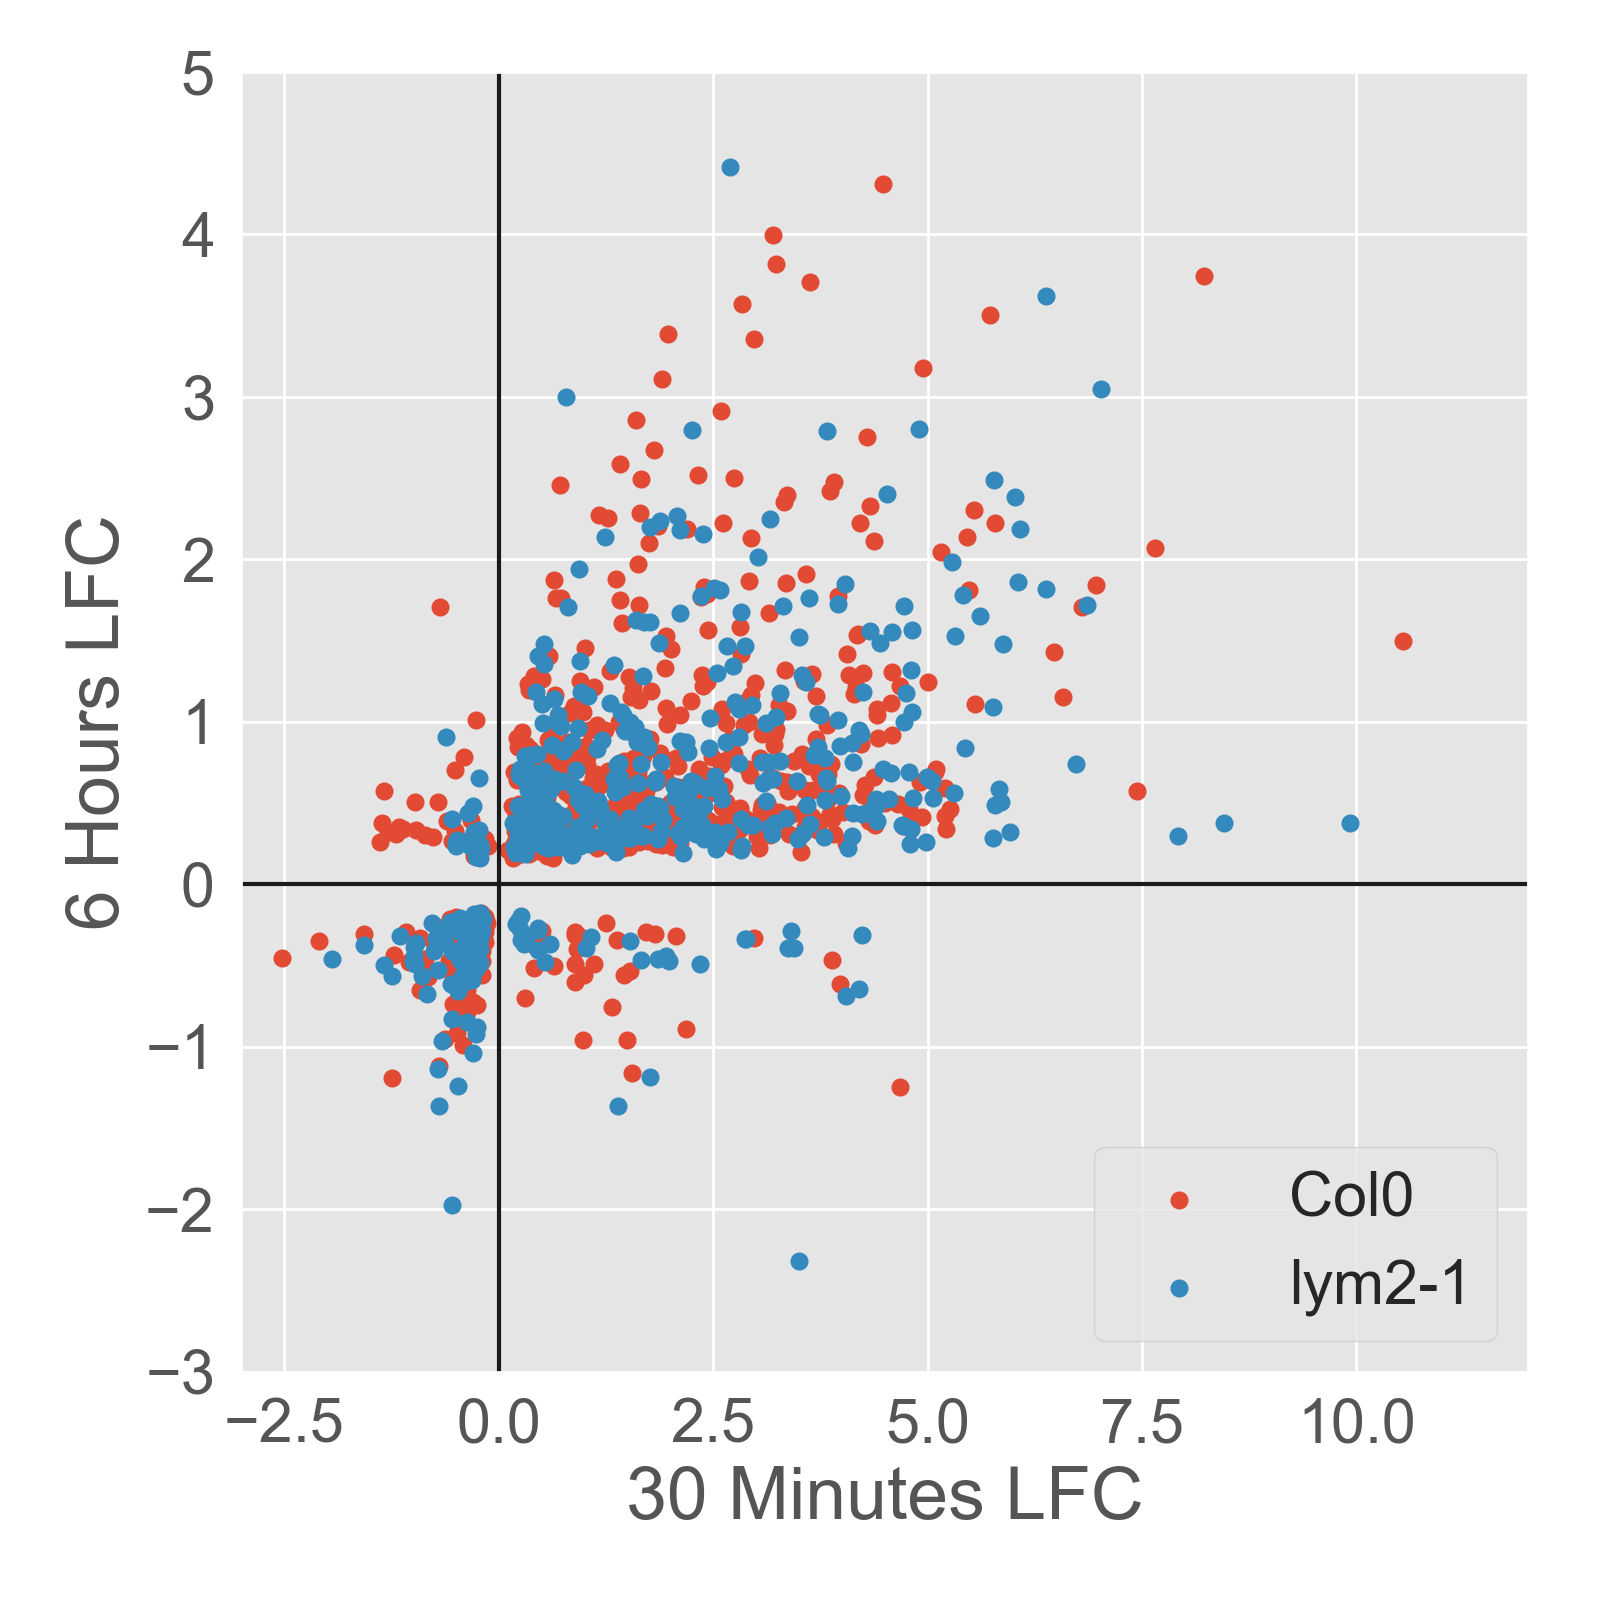
\includegraphics[width=0.5\columnwidth]{./figures/divergingGenes_all.png}
  }
  \subfloat[Genes found when selecting for opposite expression patterns\label{subfig-2:diverg}]{%
    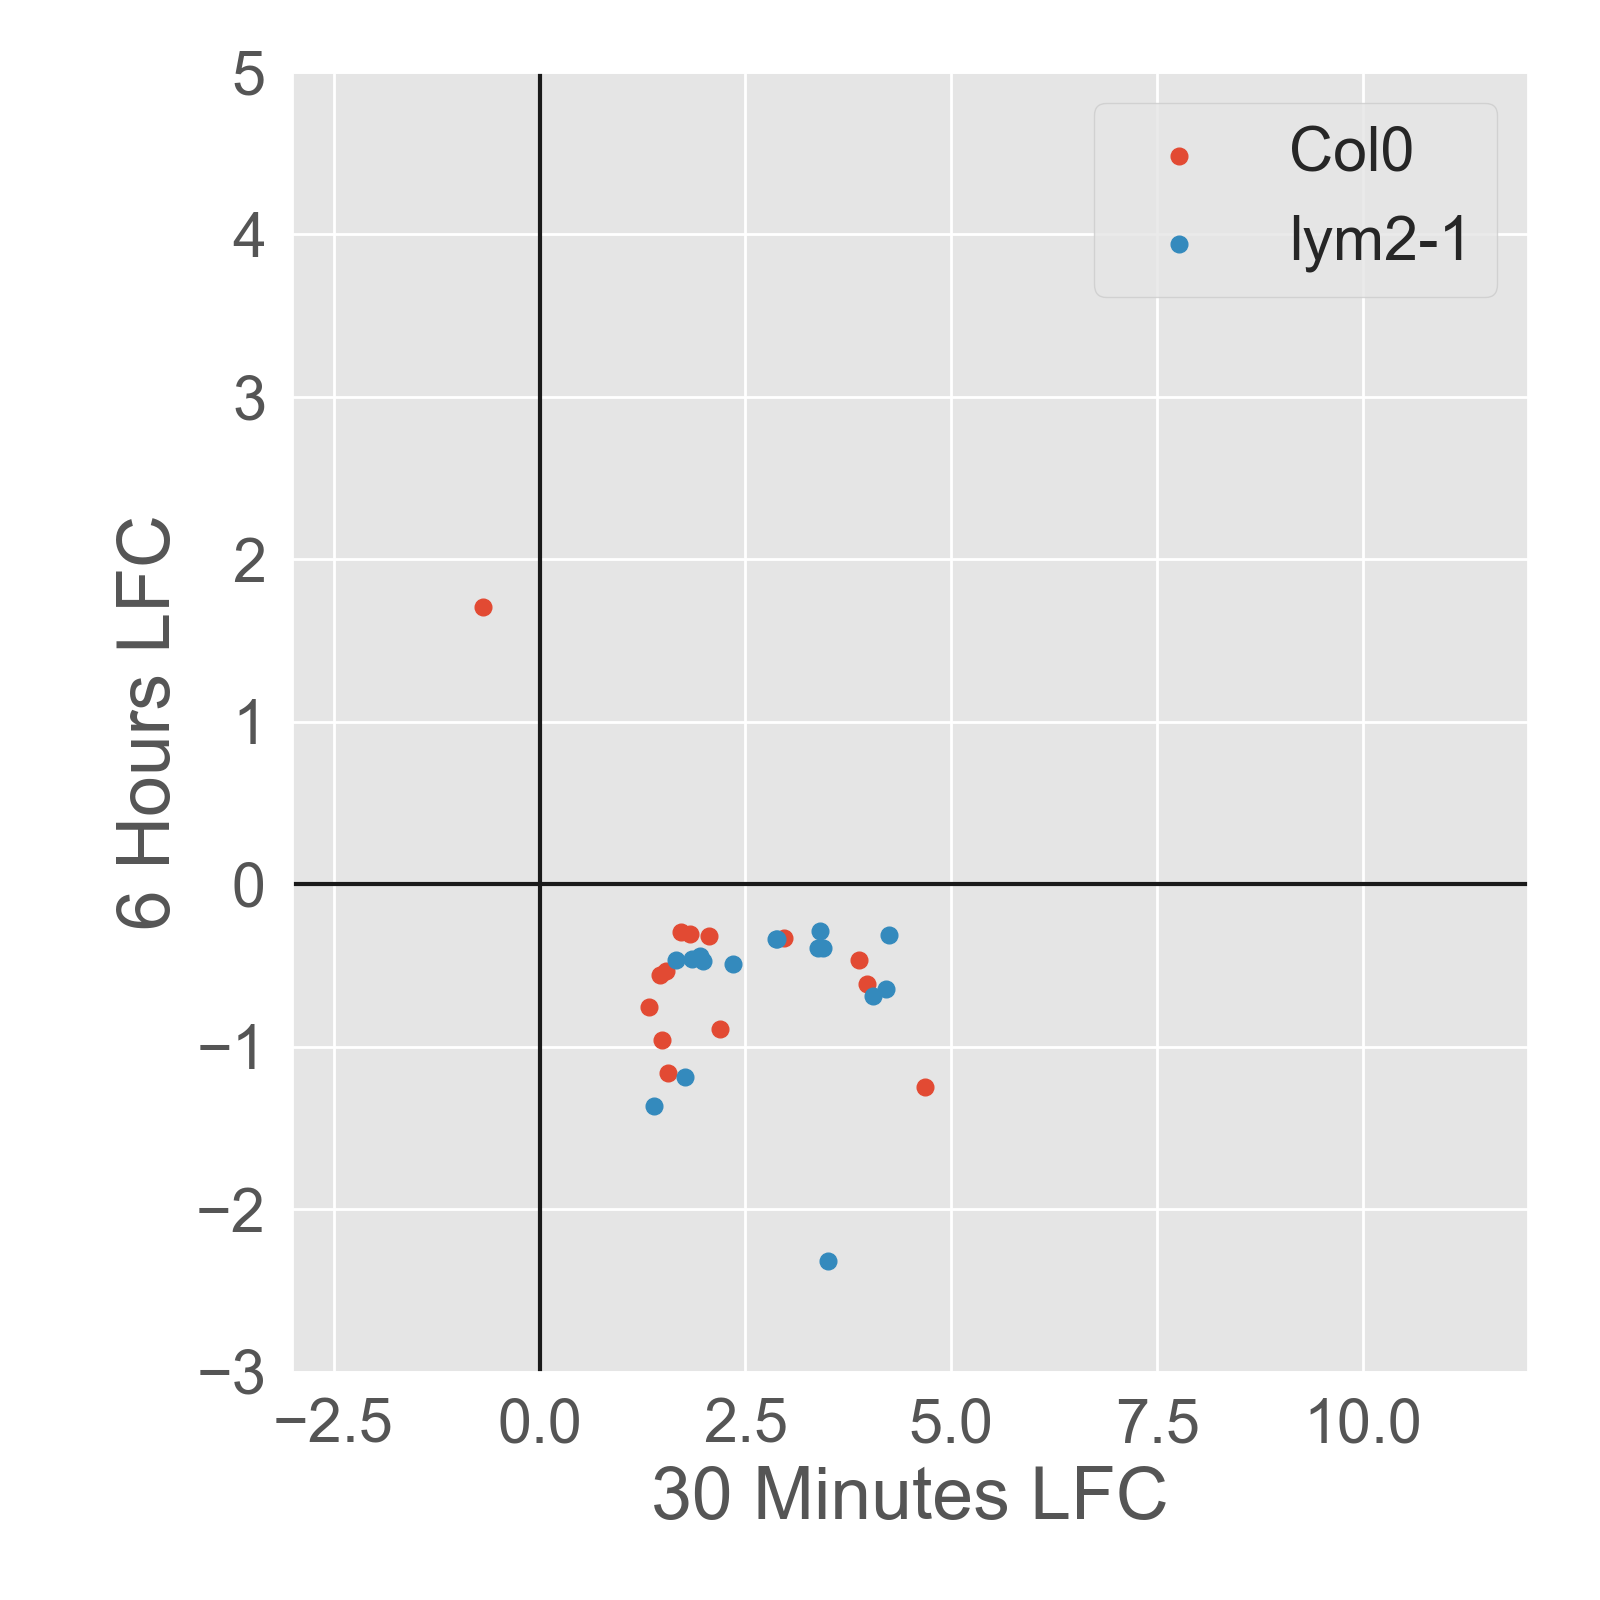
\includegraphics[width=0.5\columnwidth]{./figures/divergingGenes.png}
  }
  \caption[Differential genes plotted by expression at two time points]{DEGs plotted by time after chitin application. X axis gives
    expression at 30 minutes, Y 6 hours. Colour shows genotype, Col-0 is shown
    in red and \textit{lym2-1} in blue}
  \label{fig:diverg}
\end{figure}


\subsection{CERK1 acts as an amplification for some genes}
\label{sec:cerk1-acts-as}

For the genes we selected for their unique temporal patterning, we find two
interesting features. One, they are not documented to be defence related and two
it appears as \textit{cerk2-1} maintains directional change as Col-0 and
\textit{lym2-1}. Yet this effect is very subdued and difficult to notice
(figure: \ref{fig:interestinggenes})

\begin{figure}[!ht]
  \centering
  \subfloat[AT3G04070 (NAC DOMAIN CONTAINING PROTEIN 47)\label{subfig-2:interest}]{%
    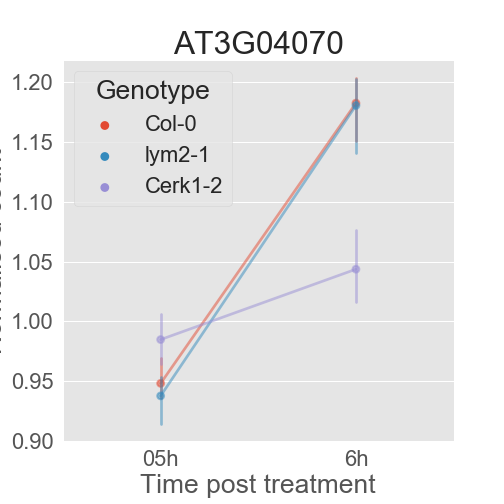
\includegraphics[width=0.7\columnwidth]{./figures/interestingGenes_AT3G04070.png}
  }\\
  \subfloat[AT5G52710 (Copper transport associated gene) \label{subfig-1:interest}]{%
    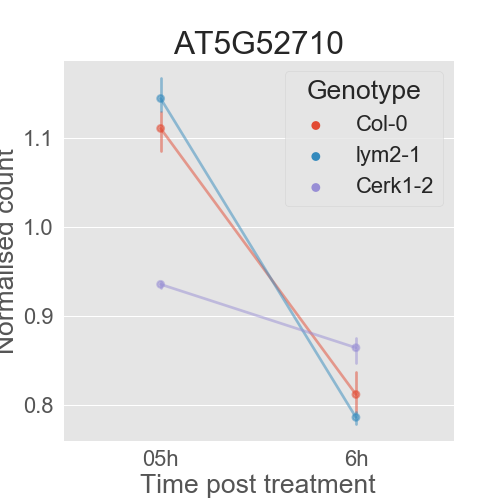
\includegraphics[width=0.7\columnwidth]{./figures/interestingGenes_AT5G52710.png}
  }
  \caption[Genes which have conflicting directions of regulation across time]{Genes which have conflicting directions of regulation across time.
    Coloured lines represent genotype, time-point on X axis, normalised
    expression count given on Y. Left plot shows expression of water control
    plants, right plot after chitin application}
  \label{fig:interestinggenes}
\end{figure}



\end{document}


%%% Local Variables:
%%% mode: latex
%%% TeX-master: "../main"
%%% End:
